\documentclass[]{article}
\usepackage{lmodern}
\usepackage{amssymb,amsmath}
\usepackage{ifxetex,ifluatex}
\usepackage{fixltx2e} % provides \textsubscript
\ifnum 0\ifxetex 1\fi\ifluatex 1\fi=0 % if pdftex
  \usepackage[T1]{fontenc}
  \usepackage[utf8]{inputenc}
\else % if luatex or xelatex
  \ifxetex
    \usepackage{mathspec}
  \else
    \usepackage{fontspec}
  \fi
  \defaultfontfeatures{Ligatures=TeX,Scale=MatchLowercase}
\fi
% use upquote if available, for straight quotes in verbatim environments
\IfFileExists{upquote.sty}{\usepackage{upquote}}{}
% use microtype if available
\IfFileExists{microtype.sty}{%
\usepackage{microtype}
\UseMicrotypeSet[protrusion]{basicmath} % disable protrusion for tt fonts
}{}
\usepackage[margin=1in]{geometry}
\usepackage{hyperref}
\hypersetup{unicode=true,
            pdftitle={Reinforcement Learning Portfolio Optimization for FX Trading},
            pdfauthor={Krzysztof Wojdalski},
            pdfborder={0 0 0},
            breaklinks=true}
\urlstyle{same}  % don't use monospace font for urls
\usepackage{longtable,booktabs}
\usepackage{graphicx,grffile}
\makeatletter
\def\maxwidth{\ifdim\Gin@nat@width>\linewidth\linewidth\else\Gin@nat@width\fi}
\def\maxheight{\ifdim\Gin@nat@height>\textheight\textheight\else\Gin@nat@height\fi}
\makeatother
% Scale images if necessary, so that they will not overflow the page
% margins by default, and it is still possible to overwrite the defaults
% using explicit options in \includegraphics[width, height, ...]{}
\setkeys{Gin}{width=\maxwidth,height=\maxheight,keepaspectratio}
\IfFileExists{parskip.sty}{%
\usepackage{parskip}
}{% else
\setlength{\parindent}{0pt}
\setlength{\parskip}{6pt plus 2pt minus 1pt}
}
\setlength{\emergencystretch}{3em}  % prevent overfull lines
\providecommand{\tightlist}{%
  \setlength{\itemsep}{0pt}\setlength{\parskip}{0pt}}
\setcounter{secnumdepth}{5}
% Redefines (sub)paragraphs to behave more like sections
\ifx\paragraph\undefined\else
\let\oldparagraph\paragraph
\renewcommand{\paragraph}[1]{\oldparagraph{#1}\mbox{}}
\fi
\ifx\subparagraph\undefined\else
\let\oldsubparagraph\subparagraph
\renewcommand{\subparagraph}[1]{\oldsubparagraph{#1}\mbox{}}
\fi

%%% Use protect on footnotes to avoid problems with footnotes in titles
\let\rmarkdownfootnote\footnote%
\def\footnote{\protect\rmarkdownfootnote}

%%% Change title format to be more compact
\usepackage{titling}

% Create subtitle command for use in maketitle
\newcommand{\subtitle}[1]{
  \posttitle{
    \begin{center}\large#1\end{center}
    }
}

\setlength{\droptitle}{-2em}

  \title{Reinforcement Learning Portfolio Optimization for FX Trading}
    \pretitle{\vspace{\droptitle}\centering\huge}
  \posttitle{\par}
    \author{Krzysztof Wojdalski}
    \preauthor{\centering\large\emph}
  \postauthor{\par}
      \predate{\centering\large\emph}
  \postdate{\par}
    \date{2018-07-21}

\usepackage[utf8]{inputenc}
\usepackage{amsthm}
\usepackage{rotating}
\pagenumbering{gobble}

\begin{document}
\maketitle

{
\setcounter{tocdepth}{3}
\tableofcontents
}
\theoremstyle{definition} \newtheorem{definition}{Definition} \newpage

\section{Abstract}\label{abstract}

The work is about reinforcement learning application in trading on the
FX market. The author starts with describing the FX market, analyzing
market organization, participants, and changes in the last years. He
tries to explain current trends and the possible directions. The next
part consists of theoretical pattern for the research - description of
financial models, and the AI algorithms. Implementation of the RL-based
approach in the third chapter, based on Q-learning, gives spurious
results.

\section{Introduction}\label{introduction}

Trading floors are usually perceived as places with noisy people and
general frenzy. This is partially justified since at some point, roughly
30 years ago, the reality was much like that. Since then the whole
industry has been evolving rapidly. Financial markets was always
interested in inventions from computer science world, it is nothing new.
Furthermore, it is part of the game - having a competitive edge in
technology helps in gaining extraordinary outcomes. The industry was
often the first one to adopt state-of-the-art technologies - increasing
efficiency is in its DNA. From sophisticated Bloomberg terminals in the
90s to blockchain and super low latency infrastructure in
2018.\footnote{Banking sector is one of the most often mentioned sector
  to adopt blockchain.}

For trading entities, as rational ones, the infinite and main goal is to
maximize its profits on the markets. One can utilize many different
approaches to achieve it and not all of them are essentially
sophisticated. In fact, one of the most famous investors ever, Warren
Buffett, still uses buy-and-hold strategy, a passive one.

In last years, though, the most emerging category of strategies are
probably the ones based on AI/machine learning paradigms. The trend is
caused by improving computation power, reducing infrastructure costs and
on top of it - the fact that humans tend to be more error-prone
{[}ref{]}. The consensus is their impact in decision making and
execution process should be assisted or even replaced by machines Turner
(2015). It is more than likely that automation of trading is going to
persist over the next years and decades. It contradicts with the cliches
mentioned at the beginning of this chapter.

Even though machine learning as a discipline is nothing new - the
fundamentals come from the 50s, the trading still has not (explicitly)
deployed it very widely. For instance, in instutional forex trading,
only a few biggest banks and sophisticated hedge funds have capabilities
to prepare efficient machine learning-based trading systems Mosic
(2017).

In the work, the author tries to explore ways in which such machine
learning (reinforcement learning) could be developed and possibly help
in gaining relatively good results.

Currently, the majority of systems described in the literature aim to
maximize trading profits or risk-adjusted measures. Although many
attempts to bring a consistently profitable system have taken place,
basing on variables inspired by econometrics of financial markets,
fundamental analysis or machine learning, most of them were not
successful due to several reasons. Among them are:

\begin{itemize}
\tightlist
\item
  Often large drawdowns - too large variability in results
\item
  High transaction costs making them impractical
\item
  High complexity - too high computation time, especially for high
  frequency trading.
\end{itemize}

Even if a given research gives an extraordinary result, once it goes to
the public, the competitive edge is going to diminish. The most
profitable strategies must be kept in secret. Otherwise, they are
useless.

\subsubsection{Work Structure}\label{work-structure}

The whole work is structured in such a way that a reader is able to
understand the whole concept of the applied reinforcement learning
algorithms. The first part consists of the detailed introduction to the
problem. It outlines the whole concept of the AI-related fields in
finance. It brought up historical background of finance and computer
sciences, and its interdependency.

The next chapter starts with the outline of selected papers from
quantitative finance. It includes both classic models, such as CAPM, the
gold standard in equity research, and modern ones. The part is
descriptive as it regards implicit pros and cons of financial models.
The literature review is specifically about algorithmic trading and the
methodology of other similar researches.

The third part is about machine learning, it is important to come up
with an explanation as to how reinforcement learning can be the best out
of known machine learning categories and in what circumstances.
Moreover, it contains comparison of most important ML groups so that a
reader can distinct them easily. The author brought up most important
concepts and aspects of RL with examples, but also potential problems,
shortcomings, limitations the algorithms are associated with.

The next part contains details of the research, such as main objectives
of the work, description of the used data, experiment design, and
finally the results. The idea was to create such agents that potentially
outperform benchmark in risk-return measures on FX market data, agents
must be robust, learn from experience, and deliver consistent results.
The chapter describes the methodology - all formulas and steps that
directed to final results. It looks at each layer of the trading system
- \#TO DO, risk management, optimization

The used algorithms are based on dynamic optimization approach. Besides
value function based on Differential Sharpe Ratio, there will be several
indicators, e.g.~RSI, which serve as a base for decision taking of the
algorithm. The methodology will include transactional costs, so that the
optimization is implemented in a real-like environment

The value function will be based by several statistics, such as the
Sharpe and the Differental Sharpe Ratio to capture both risk and return.
The algorithm output will be a set of the agents' actions in the form of
\({-1,0,1}\). In the last section of the chapter, the performance of the
trading system (RL-based agents) is demonstrated and examined against
benchmarks:

\begin{itemize}
\tightlist
\item
  Buy-and-hold strategy (holding long-position in selected currency
  pairs)
\item
  Random actions - this part of the algorithm will generate random
  values in a domain of \(\{-1,0,1\}\) . These values will serve as a
  position in the underlying pairs. The benchmark will not include any
  transactional costs as this obvious that this extreme case would have
  an enormous cumulated transactional cost (position would change in
  \(\frac{2}{3}\) of states).
\end{itemize}

The final part of the work outlines conclusion. It compares the results
with similar works and suggests possible guidelines for research
extensions. It addresses such questions as:

\begin{itemize}
\tightlist
\item
  What can be additionally implemented?
\item
  What were limitations and what must be done to avoid them in the
  future?
\end{itemize}

\subsection{FX Market Organization}\label{fx-market-organization}

Explaining the institutional structure of FX market requires introducing
formal definitions of market organization. According to Lyons Lyons
(2002), these are:

\begin{itemize}
\tightlist
\item
  Auction market - a participant can place a market and a limit order.
  The first action is aimed at buying X units at the best price.
  Alternatively, limit orders set a threshold, i.e.~they are executed
  only if the market quotations reach a certain price. Limit orders are
  aggregated into an order book
\item
  Single dealer market - in this kind of market organization, there is
  just one dealer. It is obliged to quote an asset, i.e.~to match demand
  and supply. Its quotations are always the best bid and the best ask.
  The main task is to manage the risk to make profit off his spread.
\item
  Multiple dealer market - it is extension of single dealer market.
  There is more than one dealer and they compete against each other. It
  might be centralized or decentralized. In the first version, all
  dealers are put into the same location while in the second it is not
  the case. When the market is decentralized, it is possible for price
  takers to gain profits by arbitrage transactions.
\end{itemize}

The FX market is a kind of decentralized multiple-dealer market. There
is no single indicator that would show the best bid and the best ask.
Hence, the market transparency is low. It is especially important at
tail events. It is hard to determine when the market was at a given time
and findings are usually spurious. The foreign exchange market is
perceived as the largest and most liquid one, with a year-on-year
turnover of \texteuro 69 trillion.

The FX market is an over the counter, global (OTC) market,
i.e.~participants can trade currencies with relatively low level of
legal obstacles. The market core is built up by the biggest banks in the
world. Hence, the FX organization is often referred as an inter-bank
market. The participants of the FX market differ by access, spreads,
impact, turnover they generate, order size, and purpose. They can be
divided into five main groups:

\begin{itemize}
\tightlist
\item
  Central Banks - Central banks have the biggest market impact - they
  control money supply, interest and reserve rates. Through their set of
  tools, they can strengthen or weaken local currency. In the developed
  markets, their turnover is rather small due to the fact that
  intervenings in the open market happen rarely, but order size is
  usually bigger than for other four groups due to the effect they want
  to achieve.
\item
  Commercial Banks - Most of the flow in the market belongs to
  commercial banks. Although the environment in which FX trading occurs
  is highly dispersed in terms of location, over 85\% of flow is
  generated by top 15 banks, as seen in \ref{table_turnover_banks}. It
  can be observed even for currencies that the banks do not have real
  interest in. It means that in fact banks stay with flat position.
  Their role is to gain a difference between quotations from their own
  liquidity pool and their quotations for a counterparty. Hence, over
  the years, the market have changed dramatically. Even though turnovers
  are higher than ten years, market practitioners tend to claim that
  liquidity is much worse. It is mostly due to the fact that new
  regulation, internal and external (The Basels), have been introduced.
  Banks are required to stay with rather small positions, especially in
  non-G10 pairs. Their approach to risk is much more conservative than
  it used to be.
\item
  Non-bank Financial Institutions - In the state of new regulations,
  their market significance is on the rise, e.g.~hedge funds might serve
  as liquidity providers for banks. The non-bank financial institutions
  category is very broad and entities in it are very heterogenous
\item
  Commercial Companies - their conditions as price takers are
  significantly worse than commercial banks due to the fact they trade
  bigger size and mainly hedge their main business.
\item
  Retail Traders - their main purpose is to speculate. The conditions
  they receive from financial institutions are generally worse but it
  might not be always be the case.
\end{itemize}

\begin{longtable}[]{@{}rll@{}}
\toprule
Rank & Bank & MarketShare\tabularnewline
\midrule
\endhead
1 & Citi & 16.11\%\tabularnewline
2 & Deutsche Bank & 14.54\%\tabularnewline
3 & Barclays & 8.11\%\tabularnewline
4 & JPMorgan & 7.65\%\tabularnewline
5 & UBS & 7.3\%\tabularnewline
6 & Bank of America Merrill Lynch & 6.22\%\tabularnewline
7 & HSBC & 5.4\%\tabularnewline
8 & BNP Paribas & 3.65\%\tabularnewline
9 & Goldman Sachs & 3.4\%\tabularnewline
10 & RBS & 3.38\%\tabularnewline
11 & Societe Generale & 2.43\%\tabularnewline
12 & Standard Chartered & 2.4\%\tabularnewline
13 & Morgan Stanley & 1.97\%\tabularnewline
14 & Credit Suisse & 1.66\%\tabularnewline
15 & State Street & 1.55\%\tabularnewline
\bottomrule
\end{longtable}

In last years, there have been observed shifting towards eFX. Commercial
banks, as mentioned in the previous subsection, are subject to new
regulations. Therefore, right now they are more concerned about
increasing their turnover than benefiting off a good view (speculation).
eFX helps in this goal. It requires more technology while a number of
traditional dealers is effectively reduced. The activity require
quantitative analysts, ``quants'', who can manage pricing engines in
order to maximize profit while staying in the risk threshold. Over 4
years, eFX gained 13 percent point and in 2015 for the first time
surpassed voice trading, with 53.2\% of client flow share
JeffPatterson2015 Chung2015.

The following chapter introduces articles that correspond with the
subject of the current thesis and are considered as fundamentals of
modern finance. Specifically, the beginning contains financial market
models. The next subchapter includes basic investment effectiveness
indicators that implicitly or explicitly result from the fundamental
formulas from the first subchapter.

\subsection{Selected financial market models and
theory}\label{selected-financial-market-models-and-theory}

Works considered as a fundament of quantitative finance and investments
are Sharpe (1964), Lintner (1965), and Mossin (1966). All these authors,
almost simultaneously, formulated Capital Asset Pricing Model (CAPM)
that describes dependability between rate of return and its risk, risk
of the market portfolio, and risk premium. Assumptions in the model are
as follows:

\begin{itemize}
\tightlist
\item
  Decisions in the model regard only one period,
\item
  Market participants has risk aversion, i.e.~their utility function is
  related with plus sign to rate of return, and negatively to variance
  of portfolio rate of return,
\item
  Risk-free rate exists,
\item
  Asymmetry of information non-existent,
\item
  Lack of speculative transactions,
\item
  Lack of transactional costs, taxes included,
\item
  Market participants can buy a fraction of the asset,
\item
  Both sides are price takers,
\item
  Short selling exists,
\end{itemize}

Described by the following model formula is as follows: \[
E(R_P)=R_F+\frac{\sigma_P}{\sigma_M}\times[E(R_M)-R_F]
\] where:

\begin{itemize}
\tightlist
\item
  \(E(R_P)\) -- the expected portfolio rate of return,
\item
  \(E(R_M)\) -- the expected market rate of return,
\item
  \(R_F\) -- risk-free rate,
\item
  \(\sigma_P\) -- the standard deviation of the rate of return on the
  portfolio,
\item
  \(\sigma_M\) -- the standard deviation of the rate of return on the
  market portfolio.
\end{itemize}

\(E(R_P)\) function is also known as Capital Market Line (CML). Any
portfolio lies on that line is effective, i.e.~its rate of return
corresponds to embedded risk. The next formula includes all portfolios,
single assets included. It is also known as Security Market Line (SML)
and is given by the following equation: \[ \label{eq:erl}
E(R_i)=R_F+\beta_i\times[E(R_M)-R_F]
\] where:

\begin{itemize}
\tightlist
\item
  \(E(R_i)\) -- the expected \(i\)-th portfolio rate of return,
\item
  \(E(R_M)\) -- the expected market rate of return,
\item
  \(R_F\) -- risk-free rate,
\item
  \(\beta_i\) -- Beta factor of the \(i\)-th portfolio.
\end{itemize}

\subsection{The Modern Portfolio
Theory}\label{the-modern-portfolio-theory}

The following section discuss the Modern Portfolio Theory developed by
Henry Markowitz Stulz (1995). The author introduced the model in which
the goal (investment criteria) is not only to maximize the return but
also to minimize the variance. He claimed that by combining assets in
different composition it is possible to obtain the portfolios with the
same return but different levels of risk. The risk reduction is possible
by diversification, i.e.~giving proper weights for each asset in the
portfolio. Variance of portfolio value can be effectively reduced by
analyzing mutual relations between returns on assets with use of methods
in statistics (correlation and covariance matrices). It is important to
say that any additional asset in portfolio reduces minimal variance for
a given portfolio but it is the correlation what really impacts the
magnitude. The Markowitz theory implies that for any assumed expected
return there is the only one portfolio that minimizes risk.
Alternatively, there is only one portfolio that maximizes return for the
assumed risk level. The important term, which is brought in literature,
is the effective portfolio, i.e.~the one that meets conditions above.
The combination of optimal portfolios on the bullet.

\begin{figure}
\centering
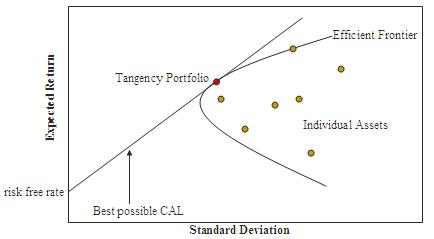
\includegraphics{../img/markowitz_frontier.jpg}
\caption{Efficient Frontier}
\end{figure}

The Markowitz concept is determined by the assumption that investors are
risk-averse. This observation is described by the following formula:

\[
E(U)<U(E(X))
\] where:

\begin{itemize}
\tightlist
\item
  \(E(U)\) -- the expected value of utility from payoff;
\item
  \(U(E(X))\) -- utility of the expected value of payoff.
\end{itemize}

The expected value of payoff is given by the following formula: \[
E(U)=\sum_{i=1}^{n}\pi_iU(c_i)
\] where:

\begin{itemize}
\tightlist
\item
  \(\pi_i\) -- probability of the \(c_i\) payoff,
\item
  \(U(c_i)\) -- utility from the \(c_i\) payoff.
\end{itemize}

One of the MPT biggest flaws is the fact that it is used for ex post
analysis. Correlation between assets changes overtime so results must be
recalculated. Real portfolio risk may be underestimated. Also, time
window can influence the results.

\subsection{Efficient Market
Hypothesis}\label{efficient-market-hypothesis}

In 1965, Eugene Fama introduced the efficient market term. Fama claimed
that an efficient market is the one that instanteneously discounts the
new information arrival in market price of a given asset. Because this
definition applies to financial markets, it determined the further
belief that it is not possible to beat the market because assets are
correctly priced. Also, if this hypothesis would be true, market
participants cannot be better or worse. Their portfolio return would be
a function of new, unpredictable information. In that respect, the only
role of an investor is to manage his assets so that the risk is
acceptable. Fama (1965)

It is highly unlikely that EMH exists in its strongest form due to
successful quantitative hedge funds that consistetly beat the markets.
For instance, Renaissance Capital hedge fund generated on average 40\%
per annum in the last 30 years Shen (2017).

Formally, Efficient Market Hypothesis states that a market is efficient
with respect to information set \(F_t\) if its impossible to make
economic profits by trading on the basis of that information set. In
other words, it is not possible to achieve any better than risk-adjusted
average rate of return. In its essence that claim is consistent with
classical price theory Weber (2012). Over time, other versions (forms)
of the EMH has been introduced - weak, semi-strong, and strong Fama, E.
F.;Malkiel (1970).

\theoremstyle{definition}

\begin{definition}{Weak Form of the EMH}
$F_t$ represents only the information contained in the past price history of the market as of time $t$
\end{definition}

What means that there is not possibility to make abnormal returns by
using the past price movements and volumes to predict the future price
movements. However, fundamental analysis might be used to generate such
results because the market is not perfect in spotting undervalued and
overvalued stocks. Hence, the participants can find profitable companies
by researching their financial statements.

\theoremstyle{definition}

\begin{definition}{Semi-Strong Form of the EMH}
$F_t$ represents all information publicly available at time $t$
\end{definition}

It states that neither technical, nor fundamental analysis cannot be
exploited for gaining superior returns, and only non-public material
information might help in above average results.

\theoremstyle{definition}

\begin{definition}{Strong Form of the EMH}
$F_t$ represents all information (public and private) known to anyone at time t.
\end{definition}

The strong form rejects the idea of any possibility to consistently
beating the market. According to this idea, any kind information, public
or non-public, is completely embedded into current financial asset
prices. In other words, there is no advantage for anyone in the market.
Returns that deviate from expected values are attributed to pure
randomness.

\subsection{Critic of strong form of the
EMH}\label{critic-of-strong-form-of-the-emh}

There are at least a few documented anomalies that contradicts with
efficient market hypothesis. For example, price/earnings (P/E) measure
can help in systematically outperforming stocks Malkiel (2003). The
neglected firm effect claims that ``uninteresting'' companies, often
ignored by market analysts are sometimes incorrectly priced, and offer
investors potentially fruitful opportunities. Another phenomenon that
cannot be explained by the strong form of EMH is so called the January
effect Haug and Hirschey (2006). According to the authors of ``The
January Effect'' working paper, returns reached in January has
predictive power for the upcoming 11 months. It persists for both small
and large cap companies.

Although the strongest form in its essence is justified, logically
correct, it is rather unlikely that it explains the reality, even due to
the effects mentioned above.

\section{Selected investment performance
measures}\label{selected-investment-performance-measures}

Introduced articles does not include any indicator that would explicitly
measure portfolio management effectiveness. Equations that result from
the authors' work are important because some of further developed
measures are CAPM-based. The most known are the Sharpe ratio, the
Treynor ratio, and the Jensen's alpha. Popularity of these indicator
comes from the fact that they are easy to understand for the average
investor. Marte (2012) In Sharpe (1966), the author introduced the
\(\frac{R}{V}\) indicator, also known as the Sharpe Ratio (\(S\)), which
is given by the following formula: \[
S_i=\frac{E(R_i-R_F)}{\sigma_i}
\] where:

\begin{itemize}
\tightlist
\item
  \(R_i\) -- the \(i\)-th portfolio rate of return,
\item
  \(R_F\) -- risk-free rate
\item
  \(\sigma_i\) -- the standard deviation of the rate of return on the
  \(i\)-th portfolio.
\end{itemize}

Treynor (Treynor1965) proposed other approach in which denominator
includes \(\beta_i\) instead of \(\sigma_i\). The discussed formula is
given by: \[
T_i=\frac{R_i-R_F}{\beta_i}
\] where:

\begin{itemize}
\tightlist
\item
  \(R_i\) -- the \(i\)-th portfolio rate of return,
\item
  \(R_F\) -- Risk-free rate
\item
  \(\beta_i\) -- Beta factor of the \(i\)-th portfolio.
\end{itemize}

Both indicators, i.e. \(S\) and \(T\) are relative measures. Their value
should be compared with a benchmark to determine if a given portfolio is
well-managed. If they are higher (lower), it means that analyzed
portfolios were better (worse) than a benchmark. The last measure, very
popular among market participants, is the Jensen's alpha. It is given as
follows: \[
\] where:

\begin{itemize}
\tightlist
\item
  \(R_i\) -- the \(i\)-th portfolio rate of return,
\item
  \(R_F\) -- Risk-free rate
\item
  \(\beta_i\) -- Beta factor of the \(i\)-th portfolio.
\end{itemize}

The Jensen's alpha is an absolute measure and is calculated as the
difference between actual and CAPM model-implied rate of return. The
greater the value is, the better for the \(i\)-th observation.

The differential Sharpe ratio - this measure is a dynamic extension of
Sharpe ratio. By using the indicator, it can be possible to capture a
marginal impact of return at time t on the Sharpe Ratio. The procedure
of computing it starts with the following two formulas: \[
A_n=\frac{1}{n}R_n+\frac{n-1}{n}A_{n-1}
\] \[
B_n=\frac{1}{n}R_n^2+\frac{n-1}{n}B_{n-1}
\] At \(t=0\) both values equal to 0. They serve as the base for
calculating the actual measure - an exponentially moving Sharpe ratio on
\(\eta\) time scale. \[
S_t=\frac{A_t}{K_\eta\sqrt{B_t-A_t^2}}
\] where:

\begin{itemize}
\tightlist
\item
  \(A_t=\eta R_t+(1-\eta)A_{t_1}\)
\item
  \(B_t=\eta R_t^2+(1-\eta)B_{t_1}\)
\item
  \(K_\eta=(\frac{1-\frac{\eta}{2}}{1-\eta})\)
\end{itemize}

Using of the differential Sharpe ratio in algorithmic systems is highly
desirable due to the following features Moody, John E.; Wu (1997):

\begin{itemize}
\tightlist
\item
  Recursive updating - it is not needed to recompute the mean and
  standard deviation of returns every time the measure value is
  evaluated. Formula for \(A_t\) (\(B_t\)) enables to very
  straightforward calculation of the exponential moving Sharpe ratio,
  just by updating for \(R_t\) (\(R_t^2\))
\item
  Efficient on-line optimization - the way the formula is provided
  directs to very fast computation of the whole statistic with just
  updating the most recent values
\item
  Interpretability - the differential Sharpe ratio can be easily
  explained, i.e.~it measures how the most recent return affect the
  Sharpe ratio (risk and reward).
\end{itemize}

The drawdown is the measure of the decline from a historical peak in an
asset. The formula is given as follows:

\[
D(T)=\max\{max_{0, t\in (0,T)} X(t)-X(\tau)\}
\]

The Sterling ratio (SR)

The maximum drawdown (MDD) at time \(T\) is the maximum of the Drawdown
over the asset history. The formula is given as follows:

\[
MDD(T)=\max_{\tau\in (0,T)}[\max_{t\in (0,\tau)} X(t)-X(\tau)]
\]

In this chapter term \textbf{machine learning} and its subfields are
explained. Discussion also contains possible applications for trading
financial instruments.

\section{Machine Learning}\label{machine-learning}

As the field evolves, there are many definitions of machine learning
sources provide. In this subchapter, the author has arbitrarly selected
definitions that accurately captures the spirit of the discipline. What
is machine learning then? The most accepted and widely used definitions
are as follows:

\begin{itemize}
\tightlist
\item
  ``Field of study that gives computers the ability to learn without
  being explicitly programmed.'' - Arthur Samuel, a pioneer in machine
  learning and computer gaming Samuel (1959)
\item
  ``A computer program is said to learn from experience \(E\) with
  respect to some class of tasks \(T\) and performance measure \(P\), if
  its performance at tasks in \(T\), as measured by \(P\), improves with
  experience \(E\).'' - Tom Mitchell, a computer scientist and E.
  Fredkin University Professor at the Carnegie Mellon University (CMU)
  Mitchell (1997)
\end{itemize}

Especially the latter is considered as an elegant and modern definition.
Less formal, but also relevant remarks, comes from two renown authors of
textbooks from the discipline:

\begin{itemize}
\tightlist
\item
  ``Pattern recognition has its origins in engineering, whereas machine
  learning grew out of computer science. However, these activities can
  be viewed as two facets of the same field\ldots{}'' - Christopher
  Bishop
\item
  ``One of the most interesting features of machine learning is that it
  lies on the boundary of several different academic disciplines,
  principally computer science, statistics, mathematics, and
  engineering. \ldots{}machine learning is usually studied as part of
  artificial intelligence, which puts it firmly into computer science
  \ldots{}understanding why these algorithms work requires a certain
  amount of statistical and mathematical sophistication that is often
  missing from computer science undergraduates.'' - Stephen Marsland
  Marsland (2009)
\end{itemize}

\begin{figure}
\centering
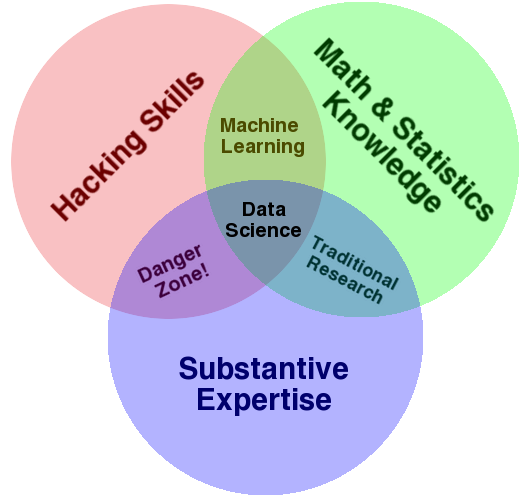
\includegraphics[height=4.16667in]{../img/data_science.png}
\caption{Data Science Graph}
\end{figure}

Altough there are many more concepts, ideas, and comments as to what
exactly machine learning is, the general goal is the same: Machine
learning is about building such models that resemble the reality to a
sufficient extent, are optimal in terms of a value function and can be
later used for predictions on new data.

\subsubsection{Why is machine learning
important?}\label{why-is-machine-learning-important}

Machine learning helps in solving problems that are difficult or even
impossible to solve in a determinisic way. Jason (2013) Sometimes
variables can be missing or observed values can contain an embedded
error. Traditional models are often prone to be under- or overdetemined.
They might not generalize well or are too general. An appropriate
machine learning model should contain approximate solution containing
only relevant parts.

\subsubsection{Classification of machine learning
algorithms}\label{classification-of-machine-learning-algorithms}

In machine learning (ML), tasks are classified into broader categories
based on how learning/feedback (\(P\)) is received and/or what kind of
problem they solve. One can distinct the following ones:

\begin{itemize}
\item
  Supervised Learning - the whole set \((Y_t;X_{t, 1}, ..., X_{t,n})\)
  is available. The goal is to model the special variable \(Y_t\) using
  a subset of \(X_t\) variables, i.e.~find a functional relationship
  \(Y_t = f(\mathbb{X_t})\) between the input variables and the output
  variables which minimizes a predefined loss function
  \(g(f(\mathbb{X}_t);Yt)\). The structural form of this relationship is
  constrained by the class of functions considered. For example we can
  assume that there is a linear relationship between input and output
  variables and a square loss function, then the problem becomes:
  \[\min_{b1\dots bn}\mathbb{E[}(Y_t-(b_1X_{t,1}+\dots+b_nX_{t,n}))^2]\]

  The utilized estimation method above is called least squares method
  for linear regression. Even though it is considered a simple one, it
  sometimes provides sufficient results. Other popular methods for
  supervised learning are:

  \begin{itemize}
  \tightlist
  \item
    K-nearest neighboors, Neural Networks,
  \item
    SVM - Support Vector Machines,
  \item
    Random Forests
  \end{itemize}
\item
  Unsupervised learning - it is the category that deals with only
  \(\mathbb{X_t}\) set. In other words, The goal is to find patterns
  among the dataset and categorize observations. The most popular
  methods are:

  \begin{itemize}
  \tightlist
  \item
    Clustering - based on finding groups of instances which are similar
    as possible to observations from the same groups while as different
    as possible to observations from other ones
  \item
    Feature extraction - this subcategory of unsupervised learning
    consists of methods for extracting relevant variables from a set of
    variables \(\mathbb{X}_t\). Often, a subset of a dataset can contain
    a similar amount of information as the original one while reducing
    dimensionality so that a model computation is much faster and
    efficient. improves the model in Occam's Razor sense.
  \item
    Anomaly detection - this type helps in identification of
    observations that are outliers and should be carefully investigated.
    Sometimes the whole variable needs to be transformed or spotted
    observations must be removed due to their invalidity.
  \end{itemize}
\item
  Reinforcement Learning - it is probably the most intuitive category of
  ML in terms of what people implicitly believe to be artificial
  intelligence. According to ({\textbf{???}}), it captures influences
  from disciplines such as engineering, economics, mathematics,
  neuroscience, psychology and computer science. Algorithms in
  reinforcement learning maximize long-term cumulated reward and
  \textbf{interacts with the environment}, i.e.~are convenient when a
  problem is not stationary.

  The two most specific features of reinforcement learning algorithms
  are trial-and-error and delayed rewards what means that this type of
  ML uses training information to evaluate the actions rather than
  instructs by giving definitive actions. This is what distinguishes
  reinforcement learning from supervised learning and is one of the
  reasons why it is considered as a subfield in ML. Moreover, it does
  not base on a training set of labeled examples. In SL, each
  observation is strictly specified as to what an algorithm should do.
  For instance if blue balls according to the model should be in blue
  basket, they will always end up there.\\
  Supervised learning goal is to generalize well on the training data so
  that the formula works also for the test data. It is important and the
  most researched area of ML nowadays, however it is not enough when
  interaction between an agent and an\\
  environment take place. In such problems an agent should learn from
  its own actions, sense states, and gain experience.

  Reinforcement learning need to be distincted from unsupervised
  learning as well. UL is focused on finding structures not explicitly
  given by collections of unlabeled datasets. It sounds similar, but it
  is far from RL, where the whole idea is to maximize sum of reward
  signals. Finding data patterns might be useful (as stated in the
  bullet point about unsupervised learning), but it does not solve a RL
  problem. Hence, the approach analyzed in the thesis should be
  considered as a next paradigm, seperated paradigm. The only feedback
  an agent receives is a scalar reward. The goal of it is to maximize
  long-run value function which consists of summed up (discounted)
  rewards in subsequent states. The goal of the agent is to learn by
  trial-and-error which actions maximize his long-run rewards. The
  environment changes stochastically and in some cases interacts with
  the agent. The agent must choose such a policy that optimizes amount
  of rewards it receives. The design must capture this fact by adjusting
  the agent so that it does not act greedily, i.e.~it should explore new
  actions instead of exploiting existing optimal (possibly suboptimal)
  solutions.
\end{itemize}

\subsection{Selected aspects of reinforcement
learning}\label{selected-aspects-of-reinforcement-learning}

In the following section the author discussed relevant aspects and
challengees of the paradigm.

\subsubsection{Exploration/exploitation}\label{explorationexploitation}

One of the most important problems in RL is the trade-off between
exploration and exploitation. To maximize cumulated rewards an agent
should take actions that worked in the past and caused bigger payoffs
(exploit). At the very beginning of learning process it never knows what
works well, though. Hence, it needs to discover desirable actions for
its state (explore). The dilemma is unresolved as of now, there are at
least a few approaches to tackle the problem, though. In the next
subsection the author presents that possible methods on the example of
Bandit problem.

\subsubsection{\texorpdfstring{\(\epsilon\)-greedy
policy}{\textbackslash{}epsilon-greedy policy}}\label{epsilon-greedy-policy}

The simplest version is to behave greedily most of the time, i.e.~an
agent selects such action (\(A_t\)) that maximizes the used value
function (e.g. \(Q_t(a)\), but sometimes, with probability of
\(\epsilon\) pick up a random action from those available, apart from
the action value estimates. Such an algorithm guarantees that every
action for every state will be explored and eventually
\(Q_t(a)=q_*(a)\). It implies that probability of choosing the most
optimal action will converge to more than \(1-\epsilon\), to near
certainty. The disadvantage of this simple method is that it says very
little of its practical effectiveness. Asymptotic guarantee might take
too long in a real environment. It can be shown that small \(\epsilon\)
causes the agent to gain more reward at initial steps, but tends to
underperform against larger \(\epsilon\) values when number of steps is
getting larger.

\subsubsection{Optimistic initial
values}\label{optimistic-initial-values}

One of the techniques to improve agent's choices is based on the idea of
encouraging the agent to explore. Why is that? If the actual reward is
smaller than initially set up action-value methods, an agent is more
likely to pick up actions that potentially can stop getting rewards that
constantly worsen value function \(q(a)\). Eventually, the system does a
lot more exploration even if greedy actions are selected all the time.

\begin{figure}
\centering
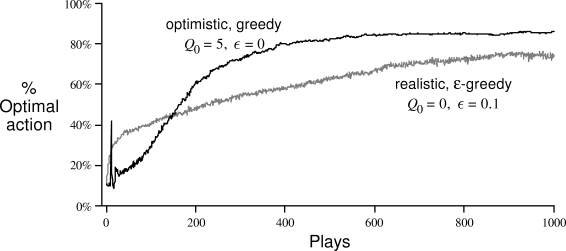
\includegraphics[height=4.16667in]{../img/optimistic_initial_values.png}
\caption{The effect of optimistic initial action-value estimates on the
10-armed testbed}
\end{figure}

\subsection{Upper-Confidence-Bound Action
Selection}\label{upper-confidence-bound-action-selection}

The other method for handling the exploration/exploitation problem is by
using the special bounds that narrow with the number of steps taken. The
formula is as follows:

\[A_t = arg\max_a[Q_t(a)+c\sqrt\frac{ln_t}{N_t(a)}\] where:

\begin{itemize}
\tightlist
\item
  \(ln_t\) is the natural logarithm of \$t\%
\item
  \$N\_t(a) - the number of times that action a has been selected prior
  to time \(t\)
\item
  \(c\) - the exploration rate
\end{itemize}

The idea of this soltuion is that the square-root part is an uncertainty
measure or variance in the \(a\) estimation. The use of the natural
logarithm implies that overtime square-root term, so does the confidence
interval, is getting smaller. All actions will be selected at some
point, but the ones with non-optimal values for \(Q(a)\) are going to be
selected much less frequently over time. UCB performs well, but it is
harder to apply (generalize) for a broader amount of problems than
\(\epsilon\)-greedy algorithm. Especially, when one is dealing with
nonstationary problems. In such situations, algorithms more complex than
those presented in this subsection should be selected.

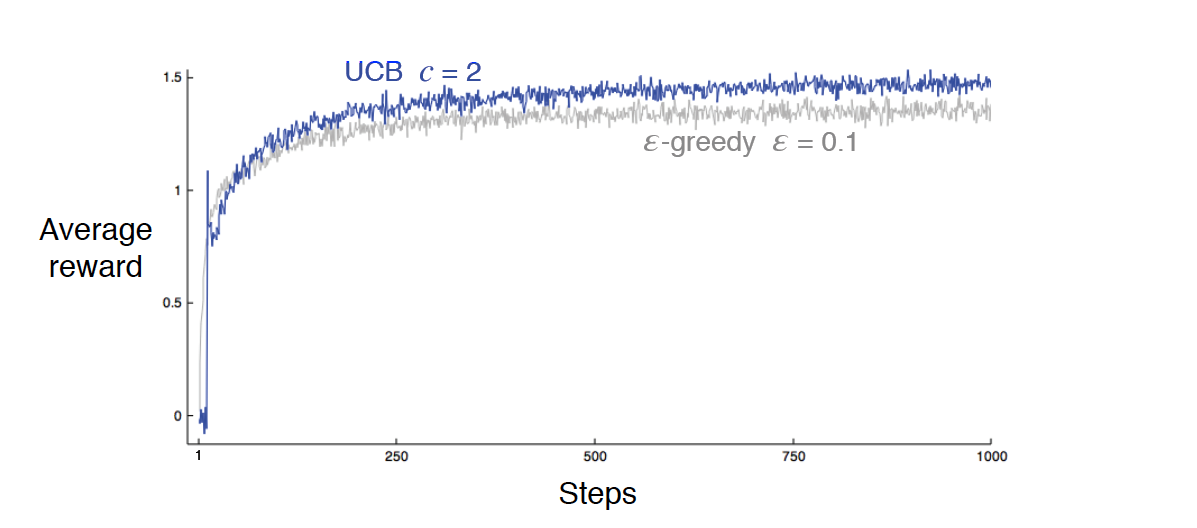
\includegraphics[height=4.16667in]{../img/ucb_vs_egreedy.png}

Reinforcement learning algorithms can be classified into three general
subcategories:

\begin{itemize}
\item
  Model Based - they are based on the idea that an model of the
  environment is known. Actions are chosen by searching and planning in
  this model. Markov Decision Process (MDP) is a typical example of such
  method since it requires knowledge of the Markov transition matrix and
  reward function.
\item
  Model-free - it uses experience to learn in a direct way from
  state-action values or policies. They can achieve the same behaviour,
  but without any knowledge on the world model an agent acts in. In
  practical examples, reinforcement learning is primarily used for
  environments where a transition matrix is not known. Given a policy, a
  state has some value, which is defined as cumulated utility (reward)
  starting from the state. Model-free methods are generally less
  efficient than model-based ones because information about the
  environment is combined with possibly incorrect estimates about state
  values Dayan and Niv (2008).
\item
  Value iteration
\item
  Policy iteration - it is an iterative method to estimate both the
  optimal value function \(V_*\) and the policy \(\pi_*\). This type of
  algorithms. The
\end{itemize}

\subsection{Components of an reinforcement learning
system}\label{components-of-an-reinforcement-learning-system}

Reinforcement learning systems are developed to solve sequential
decision making problems, to select such actions that eventually
maximize cumulative discounted future rewards. In the following section
the author explained components of reinforcement learning on the example
of game of chess and trading. The subsection was partially inspired and
based on Sutton and Barto (2017).

\begin{itemize}
\item
  Environment (\(E\)) - it defines what states and actions are possible.
  In the game of chess it is the whole set of rules and possible
  combination of figures on the chessboard. It must be stated that some
  states are not available and will be never reached. In trading such
  rules might constitute that for instance the only position an agent
  can take is 0 or 1, or that weights of assets in a portfolio must sum
  up to 1.
\item
  State (\(s\)) - can be seen as a snapshot of the environment. It
  contains a set of information in time \(t\) that a RL agent uses to
  pick the next action. States can be terminal, i.e.~the agent will no
  longer be able to choose any action. In such scenario they end an
  episode (epoch), a sequence of state-action pairs from the start to
  the end of the game. For a trading application, a state in time \(t\)
  can be a vector of different financial measures, such as rate of
  return, implied/realized volatility, moving averages, economics
  measures, technical indicators, market sentiment measures, etc.
\item
  Action (\(a\)) - givn a current state the agent chooses an action
  which directs him into a new state, either deterministically or
  stochastically. The action choice process itself may also be
  deterministic or based on probability distributions. In the game of
  chess analogy, an action is to move a figure in accordance to the
  game's rules. In trading it could be for instance going long, short,
  staying flat, outweighing.
\item
  Reward (\(r\))
\item
  Policy (\(\pi\)) - a policy is a mapping from state of the environment
  to action to be taken in that state. In psychology it is called a set
  of stimulus, i.e.~response rules or associations. The policy might be
  a lookup table or a simple function (e.g.~linear), but not
  necessarily. Especially in trading where variables are often continous
  extensive computations to set up a satisfying outcome take place. The
  policy is the most essential part of a reinforcement learning agent
  because they determine how it behaves. It may be stochastic. Policies
  do not imply deterministic nature of the mapping. Even after countless
  number of episodes and states, there is a chance that an efficient RL
  algorithm will explore other states rather than by exploiting the
  then-optimal action
\item
  Value Function - it is a prediction of future, usually discounted
  rewards. Value functions are used for determining how much a state
  should be desired by the agent. They depend on initial states
  (\(S_0\)), and a policy that is picked up by the agent. Every state
  should have an associated value, even if the path it's part of was
  never explored - in such cases they usually equal to zero. The general
  formula for value function is as follows:
\end{itemize}

\[V^\pi=\mathbb{E}_\pi[\sum\limits_{k=1}^\infty \gamma^kr_{t+k}|s_t=s]\]

where \(\gamma\) is a discount factor from the range \([0; 1]\). It
measures how much more instant rewards are valued. The smaller it is the
more immediate values are relatively more relevant and cause algorithm
to be more greedy. Sometimes \(\gamma\) is equal to 1 if it is justified
by the design of the whole agent.

\begin{itemize}
\tightlist
\item
  Model (\(m\)) - a model shows the dynamics of environment, how it will
  evolve from \(S_{t-1}\) to \(S_t\). The model helps in predicting what
  the next state and next reward will be. They are used for planning,
  i.e.~trial-and-error approach is not needed in order to achieving the
  optimal policy. Formally, it is a set of transition matrices:
\end{itemize}

\[\mathbb{P}_{ss^{'}}^a=\mathbb{P}[s^{'}|s,a]\]
\[\mathbb{R}_s^a=\mathbb{E}[r|s,a]\]

where:

\begin{itemize}
\tightlist
\item
  \(\mathbb{P}_ss^{'}{a}\) is a matrix of probability of transitions
  from state \(s\) to state \(s^{'}\) when taking action \(a\).
  Analogously, \(\mathbb{R}_{s}^a\) is an expected value of reward when
  an agent is in state \(s\) and taking action \(a\)
\end{itemize}

\subsubsection{Limitations}\label{limitations}

Reinforcement learning is not a panacea for all kinds of ML problems,
they should be heavily associated with problems based on states, some
policy to determine and defined value function. A state is just a signal
that reaches the agent, a snapshot of the environment at a time. Most of
pure reinforcement learning methods are oriented about states and their
values. Even though it is useful for simpler environments, for more
sophisticated ones it is not as easy. First of all, tabular data is not
a good way to store information about expected values for
states/states-actions. They would not fit into memory as variables are
continuous. Hence, some additional approaches must be used in order to
solving the problem efficiently.

\section{Research Objective}\label{research-objective}

The primary research goal was to evaluate the Reinforcement
Learning-based algorithm for multiasset trading. The main idea behind
the algorithm deployment is that it can systematically outperform
benchmarks in terms of selected risk and return measures. Designed
trading system was aimed to spot non-trivial patterns in data, more
efficiently than human, and exploit them accordingly.

In the project author wanted to assess the possibility of using a
reinforcement learning agent for trading domain. The objectives are as
follows

\begin{itemize}
\tightlist
\item
  Implementation - consisting of creating reinforcement learning-based
  agent that are capable of trading financial instruments basing on time
  series tables
\item
  Evaluation - testing if trading agents for out-of-sample periods can
  outperform benchmarks in the measures provided by the author
\item
  Conclusion - answering the question if such approach might help in
  generating abnormal positive results and determining if the method can
  be feasible and efficient in real-like environment
\end{itemize}

\subsection{Design of the research}\label{design-of-the-research}

The whole system can be divided into three main parts:

\begin{itemize}
\tightlist
\item
  Data preprocessing - taking FX data from Bloomberg with use of the
  dedicated API, parsing the data and adjusting it for the further
  analysis. The system is dedicated for currency trading, however with
  little adjustments it could fit in other asset classes as well.
\item
  Variable extraction - not all preprocessed currency pairs are relevant
  and worth adding. For instance, if \(USD/CNH\) is highly correlated
  with \(USD/CNY\) it is senseless to add the latter to the portfolio.
  \#TO DO
\item
  State-action space - the extracted variables, based on time series for
  currency pairs, are merged into state space
\end{itemize}

\subsubsection{Assumption}\label{assumption}

In the work, the author has assumed that:

\begin{itemize}
\tightlist
\item
  Zero slippage - the FX market is liquidity is good enough that there
  the execution price is equal to the price shown by the venue
  (Bloomberg)
\item
  Zero market impact - trades executed by the agent are not big enough
  that they can move the market and cause significant market impact
\end{itemize}

\subsection{Data Preparation}\label{data-preparation}

The original data set consisted of tick data of \textbf{52} currency
pairs in three months ( observations) between November, 2017 and March,
2018. There are 3 variables for each of them:

\begin{itemize}
\tightlist
\item
  Timestamp - usually given as a UNIX timestamp (starting from 1st of
  January of 1970) with precision of milliseconds or microseconds
\item
  Bid price - the highest price that a buyer is willing to pay for a
  given amount of a currency
\item
  Ask price - the lowest price that a seller is willing to accept for a
  given amount of a currency
\item
  Mid price - the price calculated as
  \(MID_PRICE = frac{BID_PRICE + ASK_PRICE}{2}\). Usually rounded up to
  four or five decimals (depending on currency's liquidity, value
  against a non-base currency)
\end{itemize}

The ticks were left untrasnformed. The purpose was to test the method in
a real-life environment. Hence, e.g.~aggregating would ruin the initial
idea.

Bid and ask prices are taken from Bloomberg's FXGo platform using R
Bloomberg API (RBlpapi) for 1 mio of base currency. Bloomberg covers
prices from hundreds of banks and for most currency pairs in the world.
Some of them are crossed, with use of Euro or US Dollar, for instance
\textbf{EUR/JPY} is the combination of:

\[EUR/JPY = EUR/USD\times USD/JPY\]

Sometimes pairs can effectively consist of 3 parts (legs), for instance
\textbf{PLN/MXN}: \[PLN/MXN = (USD/MXN\times EUR/USD)/(EUR/PLN)\]

Using such pairs is usually problematic and reduces reliability in
backtesting. Hence, for the purpose of the work only the most liquid
pairs, based on G10 currencies, had been used:

\begin{itemize}
\tightlist
\item
  USD - United States dollar
\item
  EUR - Euro
\item
  JPY - Japanese yen
\item
  GBP - Pound sterling
\item
  CHF - Swiss franc
\item
  AUD - Australian dollar
\item
  NZD - New Zealand dollar
\item
  CAD - Canadian dollar
\item
  SEK - Swedish krona
\item
  NOK - Norwegian krona
\end{itemize}

In eFX the crucial element is spread, calculated as the difference
between bid and ask prices. It depends on several factors, such as time
of the day, one-off events, volatility, ability of liquidity providers
to warehouse risk, or market sentiment. The data source had been
selected so that it captured spread and reflected FX market as good as
possible.

Below is the glimpse of the data used in the research:

\begin{longtable}[]{@{}lrrrrr@{}}
\toprule
Index & mid & bid & ask & spread & time\_diff\tabularnewline
\midrule
\endhead
2016-11-18 22:57:31 & 1.0588 & 1.0568 & 1.0608 & 0.0040 &
NA\tabularnewline
2016-11-18 22:57:34 & 1.0586 & 1.0568 & 1.0604 & 0.0036 &
3\tabularnewline
2016-11-18 22:57:54 & 1.0588 & 1.0568 & 1.0608 & 0.0040 &
20\tabularnewline
2016-11-18 22:57:59 & 1.0586 & 1.0568 & 1.0604 & 0.0036 &
5\tabularnewline
2016-11-18 22:58:00 & 1.0588 & 1.0568 & 1.0608 & 0.0040 &
1\tabularnewline
2016-11-18 22:58:06 & 1.0590 & 1.0572 & 1.0608 & 0.0036 &
6\tabularnewline
2016-11-18 22:59:00 & 1.0592 & 1.0572 & 1.0612 & 0.0040 &
54\tabularnewline
2016-11-18 22:59:27 & 1.0586 & 1.0560 & 1.0612 & 0.0052 &
27\tabularnewline
2016-11-18 22:59:29 & 1.0590 & 1.0568 & 1.0612 & 0.0044 &
2\tabularnewline
2016-11-18 22:59:56 & 1.0595 & 1.0560 & 1.0630 & 0.0070 &
27\tabularnewline
\bottomrule
\end{longtable}

Cols: average spread (in us dollars), min spread, max spread, average
number of ticks, mid price movements

Rows: time of the day, sum

In FX market participants usually get quotations for different levels
(tiers). The assumption of the work was to use the smallest one to
reduce possible market impact.

\subsection{Code and the Research
Process}\label{code-and-the-research-process}

The implementation of trading agents was based on R (both base and
external libraries).

The graphical presentation was prepared with the use of ggplot2 library.

The R-project consists of:

\begin{itemize}
\tightlist
\item
  frun.R,
\item
  get\_data.R,
\item
  cointegration.R,
\item
  attributes.R,
\item
  discretization.R,
\item
  functions.R,
\item
  state\_space.R,
\item
  mcc.R,
\item
  q\_learning.R
\end{itemize}

The main part was based on run.R script. Running it merges all
above-mentioned scripts and executes the whole experiment.

\listoffigures

\newpage

\section*{Bibliography}\label{bibliography}
\addcontentsline{toc}{section}{Bibliography}

\hypertarget{refs}{}
\hypertarget{ref-Dayan2008}{}
Dayan, Peter, and Yael Niv. 2008. ``Reinforcement learning: The Good,
The Bad and The Ugly.''
doi:\href{https://doi.org/10.1016/j.conb.2008.08.003}{10.1016/j.conb.2008.08.003}.

\hypertarget{ref-Fama1965}{}
Fama, Eugene F. 1965. ``The Behavior of Stock-Market Prices.'' \emph{The
Journal of Business} 38 (1): 34.
doi:\href{https://doi.org/10.1086/294743}{10.1086/294743}.

\hypertarget{ref-Fama1970}{}
Fama, E. F.;Malkiel, B. G. 1970. ``Efficient capital markets: A review
of theory and empirical work.'' \emph{Journal of Finance} 25 (2):
383--417.

\hypertarget{ref-Haug2006}{}
Haug, Mark, and Mark Hirschey. 2006. ``The january effect.''
doi:\href{https://doi.org/10.2469/faj.v62.n5.4284}{10.2469/faj.v62.n5.4284}.

\hypertarget{ref-Jason2013}{}
Jason, Brownlee. 2013. ``What is Machine Learning?''
\url{https://machinelearningmastery.com/what-is-machine-learning/}.

\hypertarget{ref-Lintner1965}{}
Lintner, John. 1965. ``Security prices, risk, and maximal gains from
diversifivation.'' \emph{Jf} 20 (4): 587--615.
doi:\href{https://doi.org/10.1111/j.1540-6261.1965.tb02930.x}{10.1111/j.1540-6261.1965.tb02930.x}.

\hypertarget{ref-Lyons2002}{}
Lyons, Richard K. 2002. ``The Microstructure Approach to Exchange Rates
(a review).'' \emph{Financial Analysts Journal} 58 (5): 101--3.
doi:\href{https://doi.org/10.2469/faj.v58.n5.2475}{10.2469/faj.v58.n5.2475}.

\hypertarget{ref-Malkiel2003}{}
Malkiel, Burton G. 2003. ``The Efficient Market Hypothesis and Its
Critics.'' \emph{Journal of Economic Perspectives} 17 (1): 59--82.
doi:\href{https://doi.org/10.1257/089533003321164958}{10.1257/089533003321164958}.

\hypertarget{ref-Marsland2009}{}
Marsland, Stephen. 2009. \emph{Machine Learning: An Algorithmic
Perspective}.
doi:\href{https://doi.org/10.1111/j.1751-5823.2010.00118_11.x}{10.1111/j.1751-5823.2010.00118\_11.x}.

\hypertarget{ref-Marte2012}{}
Marte, Jonnelle. 2012. ``No Title.'' \emph{Wall Street Journal}.

\hypertarget{ref-Mitchell1997}{}
Mitchell, Tom M. 1997. \emph{Machine Learning}. 1.
doi:\href{https://doi.org/10.1145/242224.242229}{10.1145/242224.242229}.

\hypertarget{ref-MoodyWu1997}{}
Moody, John E.; Wu, L. 1997. ``Optimization of trading systems and
portfolios.'' London.

\hypertarget{ref-Mosic2017}{}
Mosic, Ranko. 2017. ``Deep Reinforcement Learning Based Trading
Application at JP Morgan Chase.'' \emph{Medium}.
\url{https://medium.com/@ranko.mosic/reinforcement-learning-based-trading-application-at-jp-morgan-chase-f829b8ec54f2}.

\hypertarget{ref-Mossin1966}{}
Mossin, Jan. 1966. ``Equilibrium in a capital asset market.''
\emph{Econometrica} 34 (4): 768--83.
doi:\href{https://doi.org/10.2307/1910098}{10.2307/1910098}.

\hypertarget{ref-Samuel1959}{}
Samuel, Arthur L. 1959. ``Some Studies in Machine Learning Using the
Game of Checkers Some Studies in Machine Learning Using the Game of
Checkers.'' \emph{IBM Journal} 3.
\href{https://www.cs.virginia.edu/\%7B~\%7Devans/greatworks/samuel1959.pdf}{https://www.cs.virginia.edu/\{\textasciitilde{}\}evans/greatworks/samuel1959.pdf}.

\hypertarget{ref-Sharpe1964}{}
Sharpe, William F. 1964. ``Capital Asset Prices: A Theory of Market
Equilibrium under Conditions of Risk.'' \emph{The Journal of Finance} 19
(3): 425--42.
doi:\href{https://doi.org/10.2307/2329297}{10.2307/2329297}.

\hypertarget{ref-Sharpe1966}{}
---------. 1966. ``Mutual Fund Performance.'' \emph{The Journal of
Business} 39 (S1): 119.
doi:\href{https://doi.org/10.1086/294846}{10.1086/294846}.

\hypertarget{ref-Shen2017}{}
Shen, Lucinda. 2017. ``Here's How Much the Top Hedge-Fund Manager Made
Last Year.''
\url{http://fortune.com/2017/05/16/hedge-fund-james-simons-renaissance-technologies/}.

\hypertarget{ref-Markowitz1952}{}
Stulz, Rene M. 1995. ``American Finance Association, Report of the
Managing Editor of the Journal of Finance for the Year 1994.'' \emph{The
Journal of Finance} 50 (3): 1013.
doi:\href{https://doi.org/10.2307/2329297}{10.2307/2329297}.

\hypertarget{ref-Sutton2017}{}
Sutton, R S, and A G Barto. 2017. ``Reinforcement Learning: An
Introduction.'' \emph{Neural Networks IEEE Transactions on} 9 (2): 1054.
doi:\href{https://doi.org/10.1109/TNN.1998.712192}{10.1109/TNN.1998.712192}.

\hypertarget{ref-Turner2015}{}
Turner, Matt. 2015. ``The robot revolution is coming for Wall Street
traders.''
\url{http://www.businessinsider.com/robots-to-replace-wall-street-traders-2015-8?IR=T}.

\hypertarget{ref-Weber2012}{}
Weber, Thomas A. 2012. ``Price Theory in Economics.'' In \emph{The
Oxford Handbook of Pricing Management}.
doi:\href{https://doi.org/10.1093/oxfordhb/9780199543175.013.0017}{10.1093/oxfordhb/9780199543175.013.0017}.


\end{document}
